\documentclass[10pt, a4paper]{article}

\usepackage[a4paper, total={6.77in, 9.7in}, headheight=15pt]{geometry}
\usepackage{amsmath}
\usepackage{amssymb}
\usepackage{graphicx}
\usepackage{tikz}

\usetikzlibrary{arrows.meta, positioning, calc}

\usepackage{subcaption}
\usepackage{tabularx}
\usepackage{booktabs}
\usepackage{array}
\usepackage{longtable}
\usepackage{float}
\usepackage{lscape}
\usepackage{siunitx}
\usepackage{fancyhdr}
\usepackage{needspace}
\usepackage[british]{babel}
\usepackage[backend=biber, style=ieee]{biblatex}

\addbibresource{references.bib}

\usepackage{hyperref}
\usepackage{cleveref}

\hypersetup{hidelinks}

\fancypagestyle{plain}{
	\fancyhf{}
	\fancyhead[L]{%
		\hyperlink{title}{Evaluating Deep Learning Architectures}
	}
	\fancyhead[R]{%
		\hyperlink{execsum}{Jack P. Nainby}
	}
	\fancyfoot[C]{%
		\hyperlink{execsum}{\thepage}
	}
	\renewcommand{\headrulewidth}{0.4pt}
}
\pagestyle{fancy}
\fancyhf{}
\fancyhead[L]{%
	\hyperlink{title}{Evaluating Deep Learning Architectures}
}
\fancyhead[R]{%
	\hyperlink{execsum}{Jack P. Nainby}
}
\fancyfoot[C]{%
	\hyperlink{execsum}{\thepage}
}
\renewcommand{\headrulewidth}{0.4pt}

\let\oldsection\section
\renewcommand{\section}{%
    \Needspace{4\baselineskip}%
    \oldsection
}

\let\oldsubsection\subsection
\renewcommand{\subsection}{%
    \Needspace{4\baselineskip}%
    \oldsubsection
}

\let\oldsubsubsection\subsubsection
\renewcommand{\subsubsection}{%
    \Needspace{4\baselineskip}%
    \oldsubsubsection
}

\sisetup{round-mode = places}

\newcommand{\wraphead}[1]{\multicolumn{1}{>{\centering\arraybackslash}p{1.5cm}}{\textbf{#1}}}

\begin{document}
	
	\pagenumbering{arabic}
	
	\hypertarget{title}{}
	\begin{center}
	\Huge\mdseries Evaluating Deep Learning Architectures and Training Strategies for Facial Emotion Recognition Using the FER2013 Dataset\par
	\vspace{1cm}
	\Large Jack P. Nainby\par
	\Large BSc Data Science $\cdot$ Technical Project Report $\cdot$ Version 1.1\par
	\Large November 2026\par
	\end{center}
	
	\section*{Executive Summary}
	\phantomsection
	\hypertarget{execsum}{}
		
		This project compared four custom convolutional neural networks (CNNs) with transfer-learning configurations based on VGG16, ResNet50 and InceptionV3 for seven-class facial emotion recognition on FER2013. The $34$ configurations were each evaluated over five successful runs. Assessment included validation and test accuracy, balanced accuracy, class-level measures, confusion matrices and recorded computational performance.\\
		VGG16 configurations occupied the first eight composite-ranking positions; the highest-ranked custom CNN, \texttt{CNN\_Model\_Residual\_fnloss}, ranked ninth. The leading configuration depended on the metric: \\\texttt{VGG16\_Unfreeze4\_Weighted} had the highest mean validation accuracy ($0.5852$), \texttt{VGG16\_Unfreeze4\_Focal} the highest mean test accuracy ($0.5775$), and \texttt{VGG16\_Unfreeze4\_Head\_Weighted\_Focal} the highest Stage Two mean balanced accuracy ($0.5646$). Class weighting improved balanced accuracy and Macro F1 for the selected transfer models but reduced them for the custom CNNs; focal loss had mixed effects. Disgust and Fear remained difficult to recognise. Recorded times included evaluation and, in some cases, failed attempts and retries. Because test-derived measures contributed to selection and ranking, the test results are not an independent final assessment.
			
			
	\section{Introduction}
	
		\subsection{Project Context}
		
			Facial emotion recognition (FER) classifies facial images into predefined expression categories and has potential applications in human--computer interaction and affective computing. Such labels should not be treated as definitive evidence of a person's internal emotional state: expression and interpretation vary with the individual and context.\\
			CNNs learn visual features from image data, but their performance may depend on architecture, training strategy and dataset characteristics. Overall accuracy can conceal differences between emotion classes. This project therefore considers aggregate performance, class-level behaviour and recorded computational requirements.
		
		\subsection{Aim and Objectives}
		
			The aim was to evaluate how architectural choices and selected training strategies influenced deep-learning performance for FER on FER2013. The research question was: \textit{How do architectural design choices and training strategies influence the performance of deep learning models for facial emotion recognition on the FER2013 dataset?}\\
			Custom CNNs and transfer-learning models were compared using aggregate and class-level measures, recorded computational performance and a composite ranking. Conclusions are limited to the configurations and conditions tested.
	
	
	\section{Dataset and Preparation}
	
		\subsection{The FER2013 Dataset}
			
			FER2013 contains $48\times48$ grayscale facial images labelled as Angry, Disgust, Fear, Happy, Sad, Surprise or Neutral. The low resolution limits fine-grained visual information, and class frequencies are uneven: Happy is the most represented class and Disgust the least \cite{goodfellow2015challenges, fer2013_kaggle}.\\
			The original partitions were Training ($28,709$ images), PublicTest ($3,589$) and PrivateTest ($3,589$). They were used as the training, validation and test sets respectively, without changing the partition boundaries.\\
			Happy had $8,989$ training examples, compared with $547$ for Disgust, leaving the latter with substantially fewer examples from which to learn.
				
		\subsection{Data Preparation}
			
			Pixel strings were converted to 32-bit floats, reshaped to $48\times48$, normalised to $[0,1]$ by division by $255$, and converted to three-channel RGB inputs of shape $48\times48\times3$. Integer labels were one-hot encoded for the seven output classes. The shared pipeline used no model-specific ImageNet preprocessing or dataset-level augmentation; augmentation was included within the relevant custom CNN configurations. InceptionV3 resized its input internally to $75\times75$.
				
	
	\section{Methodology}
	
		\subsection{Experimental Design}
		
			The comparative design covered four custom CNN architectures and transfer-learning configurations based on VGG16, ResNet50 and InceptionV3. It examined architectural variation, fine-tuning, class weighting and focal loss. Transfer learning used two stages: Stage One compared nine architecture/head configurations; three selected configurations progressed to Stage Two. In total, $34$ configurations were each assessed over five successful runs with different random seeds. Figure~\ref{fig:experimental_workflow} summarises this sequence, showing the shared preparation stage, the separate custom-CNN and transfer-learning branches, and their progression to repeated-run evaluation and final comparison. The diagram also distinguishes the two-stage transfer-learning process from the custom-CNN experiments, which were evaluated across their own architectural and training variations.
		
			\begin{figure}[htbp]
				\centering
				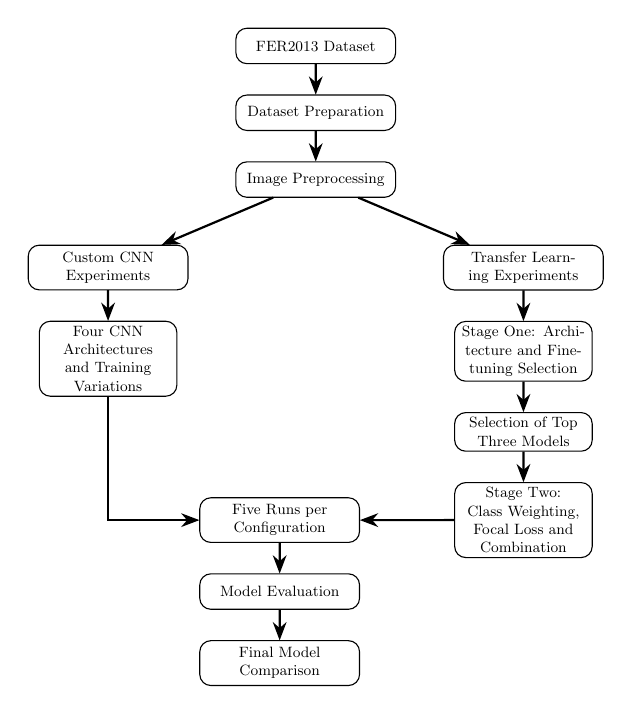
\begin{tikzpicture}[
					scale=0.60,
					transform shape,
					font=\small,
					box/.style={
						rectangle,
						rounded corners,
						draw,
						text width=3.1cm,
						minimum height=0.75cm,
						align=center,
						inner sep=4pt
					},
					smallbox/.style={
						rectangle,
						rounded corners,
						draw,
						text width=2.7cm,
						minimum height=0.7cm,
						align=center,
						inner sep=3pt
					},
					arrow/.style={-{Stealth}, thick},
					node distance=0.65cm and 1.0cm
				]

					\node[box] (dataset) {FER2013 Dataset};
					\node[box, below=of dataset] (prep) {Dataset Preparation};
					\node[box, below=of prep] (preprocess) {Image Preprocessing};

					\node[box, below left=1.0cm and 1.0cm of preprocess] (cnn){Custom CNN Experiments};

					\node[box, below right=1.0cm and 1.0cm of preprocess] (tl){Transfer Learning Experiments};

					\node[smallbox, below=of cnn] (cnnmodels){Four CNN Architectures and Training Variations};

					\node[smallbox, below=of tl] (stageone){Stage One: Architecture and Fine-tuning Selection};

					\node[smallbox, below=of stageone] (selection){Selection of Top Three Models};

					\node[smallbox, below=of selection] (stagetwo){Stage Two: Class Weighting, Focal Loss and Combination};

					\node[box, left=2.0cm of stagetwo] (runs){Five Runs per Configuration};

					\node[box, below=of runs] (evaluation){Model Evaluation};

					\node[box, below=of evaluation] (comparison){Final Model Comparison};

					\draw[arrow] (dataset) -- (prep);
					\draw[arrow] (prep) -- (preprocess);

					\draw[arrow] (preprocess) -- (cnn);
					\draw[arrow] (preprocess) -- (tl);

					\draw[arrow] (cnn) -- (cnnmodels);

					\draw[arrow] (tl) -- (stageone);
					\draw[arrow] (stageone) -- (selection);
					\draw[arrow] (selection) -- (stagetwo);

					\draw[arrow] (cnnmodels.south) |- (runs.west);
					\draw[arrow] (stagetwo.west) -- (runs.east);

					\draw[arrow] (runs) -- (evaluation);
					\draw[arrow] (evaluation) -- (comparison);

				\end{tikzpicture}
				\caption{Overview of the experimental workflow used in the investigation.}
				\label{fig:experimental_workflow}
			\end{figure}
		
		\newpage
		\subsection{Custom CNN Architectures}
				
			Four custom CNNs were evaluated: a baseline and three modified designs incorporating variations in convolutional depth and filter capacity, regularisation, augmentation and residual skip connections. The comparison concerns complete configurations; it does not isolate the contribution of each architectural change. Layer specifications are provided in the supplementary model details.
				
		\subsection{Transfer Learning Architectures}
			
			VGG16, ResNet50 and InceptionV3 were initialised with ImageNet weights and fitted with task-specific seven-class heads using global average pooling. Alternative heads with additional dense layers were also tested. InceptionV3 internally resized the shared $48\times48\times3$ input to $75\times75$.\\
			Each transfer architecture had three configurations: a frozen base, \texttt{Unfreeze4} (the final four layers trainable), and \texttt{Unfreeze4} with an additional dense head. Batch Normalisation layers in the fine-tuning group remained frozen.
				
		\subsection{Training Strategies}
			
			Class weighting adjusted each class's contribution according to its training frequency; focal loss increased the contribution of difficult examples. Custom CNNs were tested with categorical cross-entropy, weighting, focal loss, and the combination. The three modified strategies were applied to the selected transfer-learning configurations in Stage Two.
				
		\subsection{Training Procedure and Model Selection}
			
			\subsubsection{Training and Repeated Runs}
			
				Models were trained on the Training partition and monitored on PublicTest. AdamW used an initial learning rate and weight decay of $1\times10^{-4}$. EarlyStopping monitored validation loss (patience $10$) and restored the lowest-loss weights. ReduceLROnPlateau used validation loss, patience $5$, factor $0.5$ and minimum learning rate $1\times10^{-6}$. Each configuration had five successful runs with different seeds.
			
			\subsubsection{Two-stage Transfer Learning Selection}
			
				Stage One ranked the nine transfer configurations primarily by mean balanced accuracy, followed by Macro F1, mean validation accuracy, mean training time and validation-accuracy standard deviation. The selected three were \texttt{VGG16\_Unfreeze4}, \texttt{VGG16\_Unfreeze4\_Head} and \texttt{InceptionV3\_Unfreeze4\_Head}. Each progressed to Stage Two with weighting, focal loss and their combination. Because selection included test-derived measures, the test partition was not wholly independent of model selection.
			
			\subsubsection{Best-performing Run Selection}
				
				For class-level reports and confusion matrices, the run with the highest validation accuracy recorded during training was selected. This was distinct from EarlyStopping, which restored the lowest-validation-loss weights within each run. Repeated-run means were retained for aggregate comparisons.
				
		\subsection{Evaluation Measures}
			
			Assessment used validation and test accuracy, balanced accuracy, precision, recall, F1-scores and confusion matrices. Recorded time and an investigation-specific efficiency score described computational performance. A composite ranking combined eleven predictive and computational measures; it is specific to the criteria and weightings used here.
			
	
	\section{Results}
	
		\subsection{Custom CNN Results}
		
			CNN5 (the residual CNN with focal loss) gave the strongest custom-CNN results: mean validation accuracy $0.4997$, mean test accuracy $0.5053$ and mean balanced accuracy $0.4240$. CNN4 (augmentation) was close at $0.4853$, $0.4977$ and $0.4124$, with a shorter mean recorded time ($135.61$ versus $159.46$ seconds). CNN3 and the baseline achieved mean balanced accuracies of approximately $0.3499$ and $0.3152$. Selected-run Macro F1 was $0.4164$ for CNN5, $0.4155$ for CNN4, $0.3642$ for CNN3 and $0.3072$ for the baseline. These are configuration-level comparisons, not isolated tests of individual architectural changes.
		
		\subsection{Transfer Learning Results}
			
			\subsubsection{Stage One}
			
				Unfreezing the final four layers substantially improved VGG16, but effects were smaller or less consistent for ResNet50 and InceptionV3. Adding a dense head produced architecture-dependent changes: VGG16 validation accuracy rose only from $0.5837$ to $0.5846$, while balanced accuracy and Macro F1 fell; ResNet50 validation accuracy rose from $0.3466$ to $0.4169$, with balanced accuracy and Macro F1 increases of approximately $0.0752$ and $0.0903$. InceptionV3 also improved on these measures. The three configurations selected for Stage Two were \texttt{VGG16\_Unfreeze4}, \texttt{VGG16\_Unfreeze4\_Head} and \texttt{InceptionV3\_Unfreeze4\_Head}.
			
			\subsubsection{Stage Two}
				
				The leading Stage Two result depended on the measure: \texttt{VGG16\_Unfreeze4\_Head\_Weighted\_Focal} had the highest mean balanced accuracy ($0.5646$), \texttt{VGG16\_Unfreeze4\_Head\_Weighted} the highest selected-run Macro F1 ($0.5759$), \texttt{VGG16\_Unfreeze4\_Weighted} the highest mean validation accuracy ($0.5852$), and \texttt{VGG16\_Unfreeze4\_Focal} the highest mean test accuracy ($0.5775$). Class weighting increased balanced accuracy and Macro F1 for all three selected transfer configurations. For \texttt{VGG16\_Unfreeze4}, these rose from $0.4901$ to $0.5540$ and from $0.5054$ to $0.5579$; for its dense-head counterpart, from $0.4631$ to $0.5582$ and from $0.4579$ to $0.5759$. InceptionV3 also improved on both measures under each strategy. No configuration led on every measure.
				
		\subsection{Effect of Training Strategies}
		
			For custom CNNs, the strongest unweighted configuration was \texttt{CNN\_Model\_Augmentation} (test accuracy $0.4977$, balanced accuracy $0.4124$, selected-run Macro F1 $0.4155$). The strongest weighted model, \\\texttt{CNN\_Model\_Residual\_Weighted}, achieved $0.4220$, $0.4014$ and $0.3820$; the strongest focal-loss model, \\\texttt{CNN\_Model\_Residual\_fnloss}, achieved $0.5053$, $0.4240$ and $0.4164$. The combined strategy was lower ($0.4129$, $0.3903$ and $0.3709$ for \texttt{CNN\_Model\_Residual\_Weighted\_fnloss}). By contrast, class weighting improved balanced accuracy and Macro F1 for the three selected transfer configurations. Focal loss was mixed, and the combined strategy was not consistently additive. Since the strongest model under each custom-CNN strategy could differ architecturally, these comparisons do not isolate the strategy's effect.
		
		\subsection{Overall Model Comparison}
			
			\subsubsection{Classification Performance}
			
				VGG16 configurations generally outperformed the custom CNNs and other transfer architectures. The strongest custom CNN, \texttt{CNN\_Model\_Residual\_fnloss}, achieved mean test accuracy $0.5053$ and balanced accuracy $0.4240$. Macro F1 gave a different ordering: the selected run for \texttt{CNN\_Model\_Residual} scored $0.4512$, above $0.4164$ for \texttt{CNN\_Model\_Residual\_fnloss}. The measures therefore describe different aspects of performance. Figure~\ref{fig:val_vs_test} provides a visual comparison of mean validation and test accuracy for all 34 configurations. Most points lie relatively close to the dashed equality line, indicating broadly similar validation and test accuracy, although some configurations show a larger difference between the two. The higher-performing VGG16 configurations cluster towards the upper-right of the plot, while the weaker baseline variants appear towards the lower-left. The scatter therefore supports the overall performance pattern, while also showing that validation accuracy does not translate identically into test accuracy for every configuration.
				
				\begin{figure}[h!]
					\centering
					\caption{Relationship between mean validation accuracy and mean test accuracy across all 34 model configurations. The dashed reference line represents equal validation and test accuracy.}
					\label{fig:val_vs_test}
					\includegraphics[width=0.75\textwidth]{D:/GitHub/CNN-vs-transfer-learning-emotion-recognition/Results_Scatter_plot_1.png}
				\end{figure}
				
				\setlength{\tabcolsep}{3pt}
				\begin{table}[h!]
					\centering
					\caption{Best-performing Configurations Across the Evaluation Metrics}
					\label{tab:best_models}
					\makebox[\textwidth]{
					\begin{tabular}{
						l
						S[table-format=1.4, round-precision=4]
						S[table-format=1.4, round-precision=4]
						S[table-format=1.4, round-precision=4]
						S[table-format=1.4, round-precision=4]
					}
						\toprule
						Model & 
						\multicolumn{1}{>{\centering\arraybackslash}p{2cm}}{Mean Val. Acc.} &
						\multicolumn{1}{>{\centering\arraybackslash}p{2cm}}{Mean Test Acc.} &
						\multicolumn{1}{>{\centering\arraybackslash}p{2cm}}{Mean Bal. Acc.} & 
						\multicolumn{1}{>{\centering\arraybackslash}p{2cm}}{Macro F1}\\
						\midrule
						VGG16\_Unfreeze4\_Weighted & 0.585232663 & 0.55959878 & 0.554013383 & 0.557947076 \\
						VGG16\_Unfreeze4\_Focal & 0.569629419 & 0.577542496 & 0.533399107 & 0.549570798 \\
						VGG16\_Unfreeze4\_Head\_Weighted & 0.583728051 & 0.556812477 & 0.558162645 & 0.575919639 \\
					VGG16\_Unfreeze4\_Head\_Weighted\_Focal & 0.563499582 & 0.570242417 & 0.564552468 & 0.567457915 \\
						CNN\_Model\_Residual\_fnloss & 0.499749231 & 0.505321825 & 0.423987698 & 0.416388939 \\
						\bottomrule
					\end{tabular}}
				\end{table}
			
			\subsubsection{Class-level Performance}
			
				Happy and Surprise were generally recognised more successfully than Disgust and Fear. Figure~\ref{fig:confusion_matrices} compares the selected-run confusion matrices for a weighted/focal-loss VGG16 configuration, the residual CNN with focal loss, and the weighted/focal-loss baseline CNN. The rows show the proportion of each actual class assigned to each predicted class, so the diagonal entries correspond to class recall. In the VGG16 matrix (Figure~\ref{fig:cm_vgg16_unfreeze4_head_weighted_focal}), recall was highest for Happy ($71.0\%$) and Surprise ($67.5\%$), while Fear was lowest ($37.9\%$). Disgust recall was $56.4\%$, with a further $21.8\%$ of actual Disgust images classified as Angry. This gives a more detailed view of the selected VGG16 run than its aggregate accuracy alone.\\
				The residual CNN matrix (Figure~\ref{fig:cm_residual_focal}) shows a different pattern: Happy ($78.3\%$) and Surprise ($72.6\%$) were recognised relatively well, but Disgust recall was only $1.8\%$ and Fear recall $13.3\%$. In particular, $54.5\%$ of actual Disgust images were classified as Angry. The baseline matrix (Figure~\ref{fig:cm_base_weighted_focal}) shows weaker recognition across most classes, with diagonal values of $7.2\%$ for Fear, $10.4\%$ for Angry and $20.0\%$ for Disgust; Happy and Surprise were its strongest classes at $50.9\%$ and $51.2\%$. Taken together, the matrices illustrate that aggregate performance can conceal substantial class-level differences, and that the training strategies did not resolve the same weaknesses across architectures. These are selected-run results, not averages across the five runs. The residual CNN's Disgust precision of $1.0000$ should also be interpreted cautiously: it resulted from very few Disgust predictions, despite the extremely low recall.
				
				\begin{figure}[h!]
					\centering
					\caption{Representative Confusion Matrices}
					\label{fig:confusion_matrices}
					\begin{subfigure}[b]{0.32\textwidth}
						\centering
						\includegraphics[width=0.95\textwidth]{D:/GitHub/CNN-vs-transfer-learning-emotion-recognition/Plots/confusion_matrices/VGG16_Unfreeze4_Head_Weighted_Focal_confusion_matrix.png}
						\caption{VGG16}
						\label{fig:cm_vgg16_unfreeze4_head_weighted_focal}
					\end{subfigure}
					\hfill
					\begin{subfigure}[b]{0.32\textwidth}
						\centering
						\includegraphics[width=0.95\textwidth]{D:/GitHub/CNN-vs-transfer-learning-emotion-recognition/Plots/confusion_matrices/CNN_Model_Residual_fnloss_confusion_matrix.png}
						\caption{Residual CNN}
						\label{fig:cm_residual_focal}
					\end{subfigure}
					\hfill
					\begin{subfigure}[b]{0.32\textwidth}
						\centering
						\includegraphics[width=0.95\textwidth]{D:/GitHub/CNN-vs-transfer-learning-emotion-recognition/Plots/confusion_matrices/Base_CNN_Model_Weighted_fnloss_confusion_matrix.png}
						\caption{Base CNN}
						\label{fig:cm_base_weighted_focal}
					\end{subfigure}
				\end{figure}
			
			\newpage
			\subsubsection{Composite Ranking}
				
				The composite ranking combined eleven measures: mean validation, test and balanced accuracy; mean epochs and recorded time; Macro precision, recall and F1; weighted F1; validation-accuracy standard deviation; and the efficiency score. A percentile-based secondary score helped distinguish configurations. \texttt{VGG16\_Unfreeze4\_Weighted} ranked first, followed by \texttt{VGG16\_Unfreeze4\_Head\_Weighted} and \texttt{VGG16\_Unfreeze4}. VGG16 occupied the first eight positions; \texttt{CNN\_Model\_Residual\_fnloss} and \texttt{CNN\_Model\_Residual} ranked ninth and tenth. The two residual models had equal rank scores but different secondary scores. This is an investigation-specific ordering, not a universal measure of quality. Importantly, Macro F1 in the comparison table is from each selected best-run report, not a five-run mean; the accuracy and balanced-accuracy columns are repeated-run means.
				\texttt{VGG16\_Unfreeze4\_Weighted} ranked first, followed by \texttt{VGG16\_Unfreeze4\_Head\_Weighted} and \texttt{VGG16\_Unfreeze4}. VGG16 configurations occupied the first eight positions, while \texttt{CNN\_Model\_Residual\_fnloss} and \\\texttt{CNN\_Model\_Residual} ranked ninth and tenth. The two residual CNNs received identical rank scores but different weighted secondary scores, resulting in different final positions.\\
				This ranking is specific to the measures and weightings adopted in the investigation, rather than a standard or universal measure of model quality. It should therefore be interpreted alongside the individual results. Macro F1 also requires a distinction: the values in the overall comparison were taken from each configuration's selected best-run classification report, rather than calculated as means across five runs. The mean validation, test and balanced-accuracy results summarise repeated runs, whereas these Macro F1 values describe selected best runs.
				
		\subsection{Computational Performance}
			
			Mean recorded times ranged from $39.17$ seconds (\texttt{VGG16\_Unfreeze4}) to $565.01$ seconds (\texttt{ResNet50\_Frozen}). Architecture-group means were $102.27$ seconds for VGG16, $184.25$ for custom CNNs, $253.54$ for InceptionV3 and $456.43$ for ResNet50. The frozen VGG16 configuration increased its group mean.\\
			The efficiency score divided mean balanced accuracy by mean recorded time. \texttt{VGG16\_Unfreeze4} scored highest ($0.0125$; balanced accuracy $0.4901$, time $39.17$ seconds). \texttt{VGG16\_Unfreeze4\_Weighted} scored $0.0121$ with higher balanced accuracy ($0.5540$) at $45.95$ seconds. The Stage Two balanced-accuracy leader scored $0.0080$ ($0.5646$ balanced accuracy; $70.22$ seconds). Recorded time included model creation, compilation, fitting, evaluation and, where applicable, failed OOM attempts and retries. It is therefore not pure fitting time; memory, energy and inference latency were not systematically measured.
	
	
	\section{Discussion and Limitations}
	
		\subsection{Interpretation of the Main Findings}
		
			Under these conditions, transfer learning, particularly VGG16, generally outperformed the custom CNNs. No configuration led on every measure, and overall accuracy alone concealed class-level differences. Architectural complexity and imbalance-oriented training strategies did not produce uniformly positive effects; outcomes depended on the configuration. These findings apply to the models and procedures tested, not to all FER settings.
		
		\subsection{Architectural and Training Strategy Findings}
		
			The transfer-learning results differed across the three pretrained architectures. VGG16 generally produced the strongest results, but the experiment did not inspect learned features and cannot establish why. CNN4 and CNN5 outperformed the baseline and CNN3, but several design features changed together, so gains cannot be attributed to depth, capacity or residual connections alone. Class weighting and focal loss also had architecture-dependent effects.
		
		\subsection{Class Imbalance and Difficult Emotion Classes}
		
			Disgust was substantially underrepresented, which may contribute to its low recall; overall accuracy can be dominated by more frequent classes. Fear also remained difficult despite having more examples, so frequency alone cannot explain class-level performance. Differences may also reflect overlapping visual features, expression intensity and ambiguity in single-label annotations; the experiment cannot determine their individual contributions.
		
		\subsection{Evaluation Considerations}
		
			Balanced accuracy and macro-averaged measures complemented accuracy by reflecting performance across classes. The composite ranking provided a structured comparison, but depended on the selected measures and weightings. Five runs offered some indication of variability, although more repetitions would strengthen the comparison. Mean validation accuracy, test accuracy and balanced accuracy summarise repeated runs; classification reports, confusion matrices and tabled Macro F1 describe the selected run, chosen by maximum validation accuracy. They are not averages across runs. Moreover, test-derived measures contributed to Stage One selection and the overall ranking. The test partition was not used for gradient updates, but it was not an untouched final assessment.
		
		\subsection{Limitations}
			
			Only FER2013 was used. Its low-resolution grayscale images limit fine detail, while variation in appearance, expression intensity, pose, illumination and image quality may affect classification. Single categorical labels may not capture ambiguity or differences in human interpretation. Disgust was particularly underrepresented. Weighting and focal loss did not remove class-level differences, so the results should not be assumed to transfer to a more balanced or differently composed dataset.\\
			Stage Two tested training strategies only on the three Stage One selections; no ResNet50 configuration progressed. The experiments were not a complete factorial design, so independent effects and interactions between architecture, fine-tuning, head design and training strategy cannot be isolated. Five runs provide limited evidence of variability; more runs and statistical testing would be needed to assess small differences.\\
			The experiments used an RTX $3070$ GPU with $8$ GB VRAM and a Docker RAM limit of $24$ GB. Out-of-memory failures led to retries with smaller batch sizes, so successful runs did not always use identical batch sizes. Recorded time included model creation, compilation, fitting, evaluation and retries. Peak memory, energy and inference latency were not systematically measured.\\
			Generalisability was not tested on independent datasets or real-world recording conditions. Changes in image quality, illumination, appearance and class distribution may alter performance. Test-derived measures also contributed to selection, so reported test results are comparative evidence within this experiment, not an untouched estimate of generalisation.\\
			The models reproduce FER2013 labels; this does not establish that they identify a person's actual emotional or psychological state. Facial expressions do not necessarily correspond directly to internal states, and broader application risks were not evaluated. The results therefore do not establish suitability for real-world use.
	
	
	\section{Conclusion and Future Work}
	
		\subsection{Conclusion}
		
			The investigation compared four custom CNNs with VGG16, ResNet50 and InceptionV3 transfer-learning configurations across $34$ configurations and five successful runs. VGG16 occupied the first eight composite-ranking positions, and \texttt{CNN\_Model\_Residual\_fnloss} was the highest-ranked custom CNN. The leading model varied by metric, while Disgust and Fear remained difficult classes. Class weighting and focal loss had architecture-dependent effects. The findings answer the research question for the configurations and conditions tested; they do not establish a universally superior architecture or strategy.
		
		\subsection{Future Work}
			
			Selected models could be evaluated on an independent dataset, such as FER+, provided its annotations are mapped using a defined protocol. Independently collected images could test performance under different recording conditions and class distributions.\\
			Further experiments could compare additional pretrained and custom architectures while controlling input resolution, head design and fine-tuning depth. Balanced sampling, class-balanced losses and dynamic clustering could be tested alongside weighting and focal loss, with particular attention to Disgust and Fear.\\
			More independent runs and statistical comparisons could test whether observed differences are consistent. Hyperparameter optimisation could examine learning rate, batch size, dropout and fine-tuning depth, with validation data used for selection and an independent test set reserved for final assessment. Future runtime studies should separate fitting from evaluation and retry overhead, and measure peak memory, inference latency and energy. Alternative ranking criteria could also be compared.
				
	
	\printbibliography[heading=bibintoc, title={References}]

\end{document}
